\chapter{Adaptiver Gitteralgorithmus}
Mit berechenbaren Fehlerindikatoren die Verlässlichkeits- und Effizientsabschätzungen erfüllen, folgt ein Algorithmus zur effizienteren Approximation der Differentialgleichung. Dabei entsteht eine Folge von Triangulierungen. Von Glied zu Glied werden dabei die Elemente mit den größten Indikatoren verfeinert.
\begin{algorithmus}[Lösen-Approximieren-Markieren-Verfeinern]
	Wähle $\mathscr{T}_0, \theta\in (0,1],\varepsilon_{stop}>0$. Setze $k=0$.
	\begin{itemize}
		\item[(1)] berechne Approximation $u_k\in\mathscr{S}_0^1(\mathscr{T}_k)$
		\item[(2)] berechne $\eta_T(u_k)$ für alle $T\in\mathscr{T}_k$
		\item[(3)] wenn $\eta_{\mathscr{R}}(u_k) \leq \varepsilon$ dann stopp
		\item[(4)] wähle Menge $M_k\subset\mathscr{T}_k$ sodass
		\[ \sum_{T\in M_k} \eta_T^2(u_k) \geq \theta\sum_{T\in\mathscr{T}_k}\eta_T^2(u_k)\]
		\item[(5)] verfeinere jedes $T\in M_k$ und anliegende Elemente, um so neue Triangulierung $\mathscr{T}_{k+1}$ zu erhalten
		\item[(6)] $k \rightarrow k + 1$ und weiter mit (1)
	\end{itemize}
\end{algorithmus}
Im Schritt (5) müssen nach dem Verfeinern der Elemente in $M_k$ noch weitere Elemente verfeinert werden, um sicher zu stellen, dass eine konforme Triangulierung ohne hängende Knotenpunkte entsteht. Dafür können verschiedene Strategien verwendet werden.
\section{Rot-Grün-Blau Verfeinerung}
\begin{algorithmus}[2d Rot-Grün-Blau Verfeinerung]
    Sei $M_k\subset \mathscr{T}_k$ Menge der zu verfeinernden Elemente.
	\begin{itemize}
		\item[(1)] Markiere alle Seiten $S \in \mathscr{S}_k$ mit $S \subset \p T\in M_k$
		\item[(2)] Markiere weitere Seiten, sodass für alle markierten Seiten $S\subset \p T$  auch die längste Seite von T
		\item[(3)] Verfeinere Elemente je nach Anzahl markierter Seiten mit  Rot-,Blau- oder Grünverfeinerung für drei, zwei oder einer Seite markiert.
	\end{itemize}
\end{algorithmus}
\begin{figure}[!htbp]
	\begin{center}
		\includegraphics[width=16cm]{pics/redref.png}
	\end{center}
	\caption{Rote, grüne und blaue Verfeinerung eines Dreiecks}
\end{figure}
\begin{figure}[!htbp]
	\begin{center}
		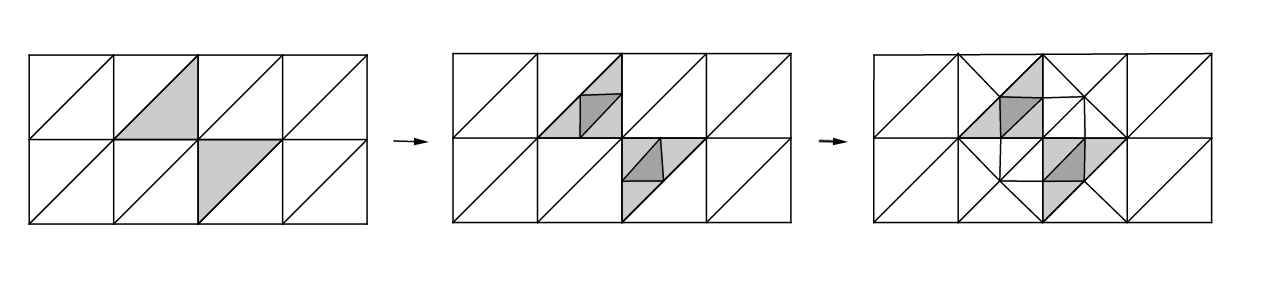
\includegraphics[width=16cm]{pics/refin.png}
	\end{center}
	\caption{Verfeinerung von markierten Elementen einer Triangulierung und weiteren Elementen, um hängende Knoten zu verhindern}
\end{figure}
\section{Bisectionsverfahren}